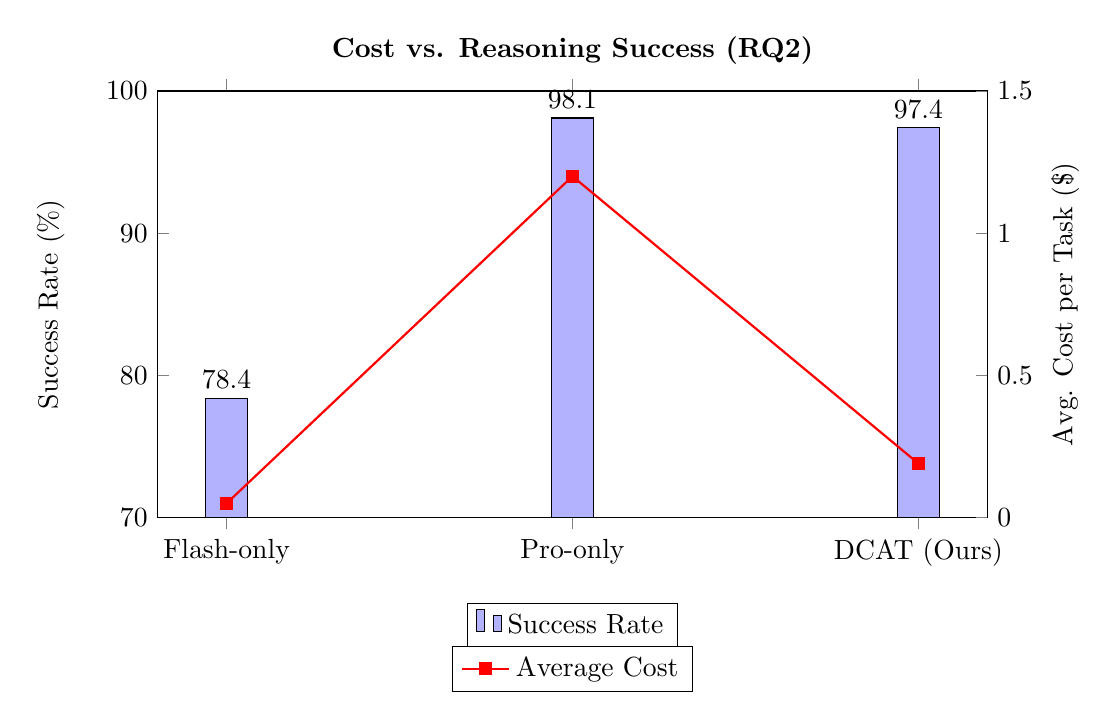
\begin{tikzpicture}
\begin{axis}[
    width=\columnwidth,
    height=7cm,
    ybar,
    bar width=15pt,
    symbolic x coords={Flash-only, Pro-only, DCAT (Ours)},
    xtick=data,
    ylabel={Success Rate (\%)},
    y label style={at={(axis description cs:-0.1,0.5)},anchor=south},
    axis y line*=left,
    ymin=70, ymax=100,
    legend style={at={(0.5,-0.2)}, anchor=north, legend columns=-1},
    nodes near coords,
    nodes near coords align={vertical},
    title={\textbf{Cost vs. Reasoning Success (RQ2)}}
]
    \addplot[fill=blue!30] coordinates {(Flash-only, 78.4) (Pro-only, 98.1) (DCAT (Ours), 97.4)};
    \legend{Success Rate}
\end{axis}

\begin{axis}[
    width=\columnwidth,
    height=7cm,
    symbolic x coords={Flash-only, Pro-only, DCAT (Ours)},
    xtick=data,
    ylabel={Avg. Cost per Task (\$)},
    axis y line*=right,
    axis x line=none,
    ymin=0, ymax=1.5,
    legend style={at={(0.5,-0.3)}, anchor=north, legend columns=-1},
]
    \addplot[sharp plot, mark=square*, red, thick] coordinates {(Flash-only, 0.05) (Pro-only, 1.20) (DCAT (Ours), 0.19)};
    \legend{Average Cost}
\end{axis}
\end{tikzpicture}
